\documentclass[a4paper]{article}
% Этот шаблон документа разработан в 2014 году
% Данилом Фёдоровых (danil@fedorovykh.ru) 
% для использования в курсе 
% <<Документы и презентации в \LaTeX>>, записанном НИУ ВШЭ
% для Coursera.org: http://coursera.org/course/latex .
% Исходная версия шаблона --- 
% https://www.writelatex.com/coursera/latex/5.3

% В этом документе преамбула

\usepackage{siunitx}
%%% Работа с русским языком
%\usepackage{cmap}					% поиск в PDF
%\usepackage{mathtext} 				% русские буквы в формулах
%\usepackage[T2A]{fontenc}			% кодировка
%\usepackage[utf8]{inputenc}			% кодировка исходного текста
%\usepackage[english,russian]{babel}	% локализация и переносы
%\usepackage{indentfirst}
%\frenchspacing
%
%\renewcommand{\epsilon}{\ensuremath{\varepsilon}}
%\newcommand{\phibackup}{\ensuremath{\phi}}
%\renewcommand{\phi}{\ensuremath{\varphi}}
%\renewcommand{\varphi}{\ensuremath{\phibackup}}
%\renewcommand{\kappa}{\ensuremath{\varkappa}}
%\renewcommand{\le}{\ensuremath{\leqslant}}
%\renewcommand{\leq}{\ensuremath{\leqslant}}
%\renewcommand{\ge}{\ensuremath{\geqslant}}
%\renewcommand{\geq}{\ensuremath{\geqslant}}
%\renewcommand{\emptyset}{\varnothing}
%\renewcommand{\Im}{\operatorname{Im}}
%\renewcommand{\Re}{\operatorname{Re}}


%%% Дополнительная работа с математикой
\usepackage{amsmath,amsfonts,amssymb,amsthm,mathtools} % AMS
%\usepackage{icomma} % "Умная" запятая: $0,2$ --- число, $0, 2$ --- перечисление

%% Номера формул
%\mathtoolsset{showonlyrefs=true} % Показывать номера только у тех формул, на которые есть \eqref{} в тексте.
%\usepackage{leqno} % Нумереация формул слева

%% Свои команды
\DeclareMathOperator{\sgn}{\mathop{sgn}}
\DeclareMathOperator{\sign}{\mathop{sign}}
\DeclareMathOperator*{\res}{\mathop{res}}
\DeclareMathOperator*{\tr}{\mathop{tr}}
\DeclareMathOperator*{\rot}{\mathop{rot}}
\DeclareMathOperator*{\divop}{\mathop{div}}
\DeclareMathOperator*{\grad}{\mathop{grad}}

%% Перенос знаков в формулах (по Львовскому)
\newcommand*{\hm}[1]{#1\nobreak\discretionary{}
{\hbox{$\mathsurround=0pt #1$}}{}}

%%% Работа с картинками
\usepackage{graphicx}  % Для вставки рисунков
\graphicspath{{figures/}}  % папки с картинками
\setlength\fboxsep{3pt} % Отступ рамки \fbox{} от рисунка
\setlength\fboxrule{1pt} % Толщина линий рамки \fbox{}
\usepackage{wrapfig} % Обтекание рисунков текстом

%%% Работа с таблицами
\usepackage{array,tabularx,tabulary,booktabs} % Дополнительная работа с таблицами
\usepackage{longtable}  % Длинные таблицы
\usepackage{multirow} % Слияние строк в таблице

%%% Теоремы
\theoremstyle{plain} % Это стиль по умолчанию, его можно не переопределять.
\newtheorem{thm}{Теорема}
\newtheorem*{thm*}{Теорема}
\newtheorem{prop}{Предложение}
\newtheorem*{prop*}{Предложение}
 
\theoremstyle{definition} % "Определение"
%\newtheorem{corollary}{Следствие}[theorem]
\newtheorem{dfn}{Определение}
\newtheorem*{dfn*}{Определение}
\newtheorem{prob}{Задача}
\newtheorem*{prob*}{Задача}

 
\theoremstyle{remark} % "Примечание"
\newtheorem*{sol}{Решение}
\newtheorem*{rem}{Замечание}

%%% Программирование
\usepackage{etoolbox} % логические операторы

%%% Страница
%\usepackage{extsizes} % Возможность сделать 14-й шрифт
%\usepackage{geometry} % Простой способ задавать поля
%	\geometry{top=25mm}
%	\geometry{bottom=35mm}
%	\geometry{left=35mm}
%	\geometry{right=20mm}
 
\usepackage{fancyhdr} % Колонтитулы
%	\pagestyle{fancy}
 %	\renewcommand{\headrulewidth}{0pt}  % Толщина линейки, отчеркивающей верхний колонтитул
	%\lfoot{Нижний левый}
	%\rfoot{Нижний правый}
	%\rhead{Верхний правый}
	%\chead{Верхний в центре}
	%\lhead{Верхний левый}
	%\cfoot{Нижний в центре} % По умолчанию здесь номер страницы

\usepackage{setspace} % Интерлиньяж
%\onehalfspacing % Интерлиньяж 1.5
%\doublespacing % Интерлиньяж 2
%\singlespacing % Интерлиньяж 1

\usepackage{lastpage} % Узнать, сколько всего страниц в документе.

\usepackage{soul} % Модификаторы начертания

\usepackage{hyperref}
\usepackage[usenames,dvipsnames,svgnames,table,rgb]{xcolor}
\hypersetup{				% Гиперссылки
    unicode=true,           % русские буквы в раздела PDF
    pdftitle={Заголовок},   % Заголовок
    pdfauthor={Автор},      % Автор
    pdfsubject={Тема},      % Тема
    pdfcreator={Создатель}, % Создатель
    pdfproducer={Производитель}, % Производитель
    pdfkeywords={keyword1} {key2} {key3}, % Ключевые слова
%    colorlinks=true,       	% false: ссылки в рамках; true: цветные ссылки
    %linkcolor=red,          % внутренние ссылки
    %citecolor=black,        % на библиографию
    %filecolor=magenta,      % на файлы
    %urlcolor=cyan           % на URL
}

\usepackage{csquotes} % Еще инструменты для ссылок

%\usepackage[style=apa,maxcitenames=2,backend=biber,sorting=nty]{biblatex}

\usepackage{multicol} % Несколько колонок

\usepackage{tikz} % Работа с графикой
\usepackage{pgfplots}
\usepackage{pgfplotstable}
%\usepackage{coloremoji}
\usepackage{floatrow}
\usepackage{subcaption}
\graphicspath{{figures/}}

\renewcommand\thesubfigure{\asbuk{subfigure}}
%\addbibresource{master.bib}

\usepackage{import}
\usepackage{pdfpages}
\usepackage{transparent}
\usepackage{xcolor}
\usepackage{xifthen}

\newcommand{\incfig}[2][1]{%
    \def\svgwidth{#1\columnwidth}
    \import{./figures/}{#2.pdf_tex}
}
%\usepackage{titlesec}
%\titleformat{\section}{\normalfont\Large\bfseries}{}{0pt}{}
%----------------------STANDART:
%\titleformat{\chapter}[display]
%  {\normalfont\huge\bfseries}{\chaptertitlename\ \thechapter}{20pt}{\Huge}
%\titleformat{\section}{\normalfont\Large\bfseries}{\thesection}{1em}{}
%\titleformat{\subsection}
%  {\normalfont\large\bfseries}{\thesubsection}{1em}{}
%\titleformat{\subsubsection}
%  {\normalfont\normalsize\bfseries}{\thesubsubsection}{1em}{}
%\titleformat{\paragraph}[runin]
%  {\normalfont\normalsize\bfseries}{\theparagraph}{1em}{}
%\titleformat{\subparagraph}[runin]
%  {\normalfont\normalsize\bfseries}{\thesubparagraph}{1em}{}

\pdfsuppresswarningpagegroup=1
\pgfplotsset{compat=1.16}



%\setcounter{tocdepth}{1} % only parts,chapters,sections
%\titleformat{\subsection}{\normalfont\large\bfseries}{}{0em}{}
%\titleformat{\subsubsection}{\normalfont\normalsize\bfseries}{}{0em}{}

%\newcommand{\textover}[2]{\stackrel{\mathclap{\normalfont\mbox{#2}}}{#1}}

\author{Yaroslav Drachov\\
Moscow Institute of Physics and Technology}
%\author{Драчов Ярослав\\
%Факультет общей и прикладной физики МФТИ}
\newcommand{\veq}{\mathrel{\rotatebox{90}{$=$}}}
%\newcommand{\teto}[1]{\stackrel{\mathclap{\normalfont\tiny\mbox{#1}}}{\to}}
%\renewcommand{\thesubsection}{\arabic{subsection}}

%%\setcounter{secnumdepth}{0}

\definecolor{tabblue}{RGB}{30, 119, 180}
\definecolor{taborange}{RGB}{255, 127, 15}
\definecolor{tabgreen}{RGB}{45, 160, 43}
\definecolor{tabred}{RGB}{214, 38, 40}
\definecolor{tabpurple}{RGB}{148, 103, 189}
\definecolor{tabbrown}{RGB}{140, 86, 76}
\definecolor{tabpink}{RGB}{227, 119, 193}
\definecolor{tabgray}{RGB}{127, 127, 127}
\definecolor{tabolive}{RGB}{188, 189, 33}
\definecolor{tabcyan}{RGB}{22, 190, 207}
\pgfplotscreateplotcyclelist{colorbrewer-tab}{
{tabblue},
{taborange},
{tabgreen},
{tabred},
{tabpurple},
{tabbrown},
{tabpink},
{tabgray},
{tabolive},
{tabcyan},
}
\usepackage{csvsimple}
\usepackage{extarrows}
%\renewcommand{\labelenumii}{\asbuk{enumii})}
%\renewcommand{\labelenumiv}{\Asbuk{enumiv}}
%\newcommand{\prob}[1]{\subsubsection*{#1}}
\sisetup{output-decimal-marker = {,},separate-uncertainty = true,exponent-product = \cdot}

\usepackage{braket}
\usepackage{enumerate}
\usepackage{chngcntr}
%\counterwithin*{equation}{problem}
%\usepackage{bbold}

\newtheoremstyle{hiProb}% ⟨name ⟩ 
{3pt}% ⟨Space above ⟩1 
{3pt}% ⟨Space below ⟩1
{}% ⟨Body font ⟩
{}% ⟨Indent amount ⟩2
{\bfseries}% ⟨Theorem head font⟩
{.}% ⟨Punctuation after theorem head ⟩
{.5em}% ⟨Space after theorem head ⟩3
%{\thmname{#1} \thmnote{#3}}% ⟨Theorem head spec (can be left empty, meaning ‘normal’)⟩
{\thmnote{#3}}% ⟨Theorem head spec (can be left empty, meaning ‘normal’)⟩
\theoremstyle{hiProb} % "Определение"
%\newtheorem{hiProb}{Задача}
\newtheorem{hiProb}{}
%\usepackage{mmacells}
\newcommand{\textover}[2]{\stackrel{\mathclap{\normalfont\scriptsize\mbox{#2}}}{#1}}
\usepackage{units}
\usepackage[math]{cellspace}%
\setlength\cellspacetoplimit{2pt}
\setlength\cellspacebottomlimit{2pt}

\DeclareMathAlphabet{\mathbbold}{U}{bbold}{m}{n}

\newcommand{\normord}[1]{:\mathrel{#1}:}

\title{Неделя №13\\
Магнитный порядок в кристаллах. Спиновые волны и их квантование}
\begin{document}
	\maketitle
\begin{hiProb}[Т13-5]
\end{hiProb}
\begin{sol}
Уровни энергии иона со спином $S=1$ в магнитном
поле расщепляются на три подуровня вследствие эффекта
Зеемана, добавка к энергии $\Delta E= g \mu_B B m_S$,
где $m_S$ --- проекция спина на направление поля.
Учитывается только спиновый, а не полный момент
из-за явления <<замораживания орбитального
момента>> в кристаллах.

Средняя энергия спина $S=1$ в магнитном поле
вычисляется при помощи распределения Гиббса:

\[
E= g \mu_B B \frac{-e^{\frac{h\mu_B B}{k_BT}}+
e^{- \frac{g\mu_B B}{k_B T}}}{1+ e^{\frac{g \mu_B
B}{k_B T}}+ e^{- \frac{g \mu_B B}{k_B T}}}=-
g \mu_B B \frac{2 \sh  \frac{g \mu_B B}{k_B T}}{1+
2\ch  \frac{g \mu_B B}{k_B T}}
.\] 
Дифференцированием находим теплоёмкость (на ион)
\[
	C= \frac{dE}{dT}= k_B \left( 
	\frac{g \mu_B B}{k_B T}\right) ^2 
	\frac{4+ 2 \ch  \frac{g \mu_B B}{k_B T}}{\left( 
	1+ 2 \ch \frac{g \mu_B B}{k_B T}\right) ^2}
.\] 
Для поиска экстремума пользуемся указанием в условии
задачи.
\[
T_{\max}= \frac{g \mu_B B}{1,881k_B}\approx 2,86 \text{ К},\quad
C_{\max}\approx 0,637 k_B
.\] 
Для оценки фононного вклада при этой температуре
берём характерную температуру Дебая 300 К
\[
	\frac{C}{N}= \frac{12}{5} \pi^4 k_B \left( 
	\frac{T}{\Theta}\right) ^3 \sim 10^{-4}
	k_B
.\] 
\end{sol}
\begin{hiProb}[Т13-6]
\end{hiProb}
\begin{sol}
Преобразуем гамильтониан:
\[
	\widehat{\operatorname{H}}= J \widehat{\operatorname{\mathbf{S}}}_1 \widehat{\operatorname{\mathbf{S}}}_2=
	\frac{1}{2}J\left( 
	\left( \widehat{\operatorname{\mathbf{S}}}_1+
\widehat{\operatorname{\mathbf{S}}}_2\right) ^2- 
\widehat{\operatorname{\mathbf{S}}}_1^2-
\widehat{\operatorname{\mathbf{S}}}_2^2\right) 
.\] 
Согласно правилу сложения моментов суммарный спин
пары спинов 1/2 (речь идёт о метал-органических
комплексах меди с ионом Cu$^{2+}$ равен 0 или 1.
При $J>0$ (антиферромагнитный знак обменного интеграла)
состояние с минимальной энергией это $S=0$ 
(синглетное состояние), состояние с $S=1$ 
(триплетное, т.\:к. трёхкратно вырождено по
проекции спина) оказывается возбуждённым. Энергии
этих состояний: $E_0= - \frac{3J}{4}$, $E_1= \frac{J}{4}$. 

Для вычисления магнитной восприимчивости заметим,
что в слабом поле снимается вырождение триплетного
уровня по проекции спина
\[
	E_1(S_z)= \frac{J}{4}+2 \mu_B H S_z
,\]
для удобства вычисления удобно отсчитывать энергию
от основного состояния. Тогда для среднего
магнитного момента
\begin{multline*}
	\left<m \right> = 2\mu_B \frac{\exp \left(- \frac{J-2\mu_B H
	}{T}\right)-\exp \left(- \frac{J+2\mu_B H}{T}\right)}{1+ \exp \left( 
	- \frac{J+ 2\mu_B H}{T}\right) +
\exp \left( -\frac{J}{T} \right) +
\exp  \left( - \frac{J-2\mu_B H}{T} \right) }
\approx\\ \approx
2\mu_B \frac{e^{-J /T}}{1+ 3 e^{- J /T}}\frac{4\mu_B H}{T}= \frac{8 \mu_B ^2 H}{T} \frac{1}{e^{J /T}+3}
=H \frac{8\mu_B^2}{J} \frac{J}{T} \frac{1}{e^{J /T}+3}
,\end{multline*} 
здесь использована малость магнитного поля и оставлены
только линейные по полю члены.

Отсюда 
\[
\chi= \frac{8 \mu_B^2}{3J} \frac{J}{T} \frac{1}{
1+\frac{e^{J /T}}{3}}
,\] 
множитель $8\mu_B^2 /(3J)$ равен
магнитной восприимчивости спина $S=1$ при температуре
$T=J$.

Низкотемпературная($T\ll J$) асимптотика 
\[
\chi_{T \ll J} \approx \frac{8 \mu_B^2}{J}\frac{J}{T}
e^{- J /T}
.\] 
Для сравнения с законом Кюри-Вейса необходима в высокотемпературной асимптотике удержать члены
порядка $1 /T^2$:
\[
\chi_{CW}= \frac{C }{T+\Theta}\approx
\frac{C}{T} \left( 1- \frac{\Theta}{T} \right) 
.\] 
\[
\chi_{T \gg J}\approx \frac{8\mu_B^2}{J}\frac{J}{T}
\frac{1}{3+1 + J /T}= \frac{2\mu_B^2}{J}
\frac{J}{T} \left( 1- \frac{J}{4T} \right) 
.\] 
Здесь можно отметить, что множитель перед
скобками $2\mu_B^2 /T$ в точности равен
восприимчивости двух парамагнитных
спинов $S= 1 /2$. Из сравнения с разложением
закона Кюри-Вейса получаем $\Theta= J /4$, знак
температуры Кюри антиферромагнитный.
\begin{figure}[htpb]
	\centering
	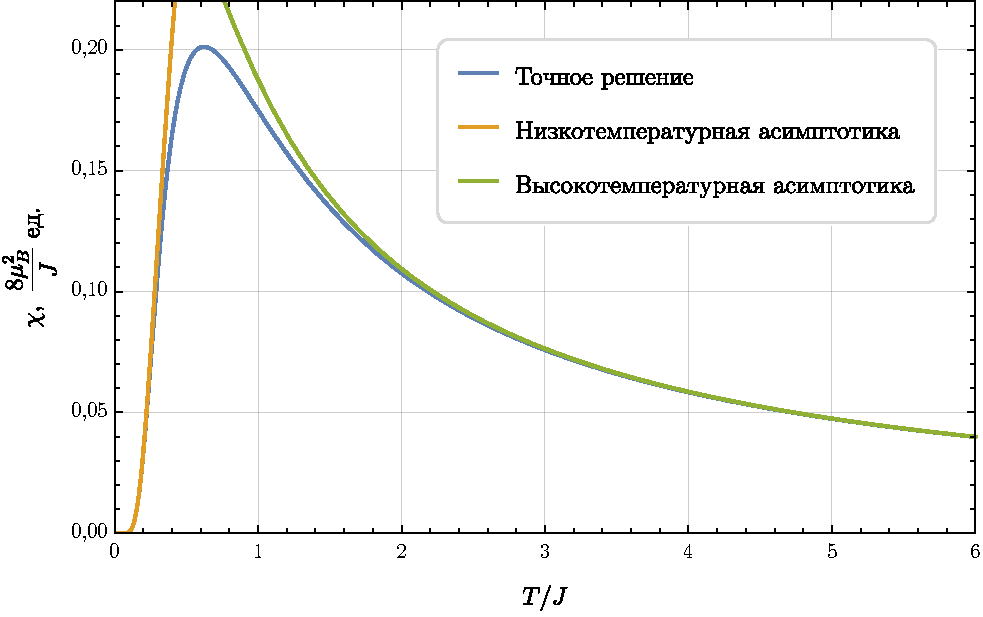
\includegraphics[width=0.8\textwidth]{1}
	\caption{Температурная зависимость магнитной
	восприимчивости антиферромагнитного димера,
к задаче Т13-6}
	\label{fig:1}
\end{figure}
\begin{figure}[htpb]
	\centering
	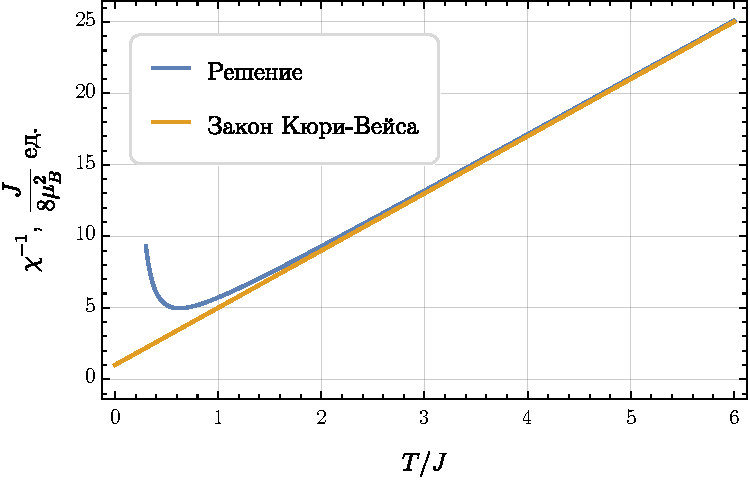
\includegraphics[width=0.8\textwidth]{2}
	\caption{График обратной восприимчивости,
		иллюстрирующий соответствие
		закону Кюри-Вейса при высоких
		температурах,
к задаче Т13-6}
	\label{fig:2}
\end{figure}
\end{sol}
\begin{hiProb}[Т13-7]
\end{hiProb}
\begin{sol}
	Для случая ферромагнетика намагниченность (на
	атом) ниже температуры Кюри описывается
	трансцендентным уравнением
	\[
	\frac{\left<m \right> }{\mu_B}=
	\tg \left( 
	\frac{\left<m \right> }{\mu_B}\frac{\Theta}{T}\right) 
	.\] 
Для условий задачи оно имеет вид
\[
\frac{1}{2}= \tg  \frac{\Theta}{2T}
.\] 
Численное решение этого уравнения $T= 0,91 \Theta$.
Тогда с использованием указания о близости к $\Theta$
можно воспользоваться разложением для
величины параметра  порядка вблизи температуры
Кюри
\[
\frac{\left<m \right> }{\mu_B}= \sqrt{3} 
\sqrt{1-\frac{T}{\Theta}} 
.\]
Тогда
\[
	\left( 1-\frac{T}{\Theta} \right) =
	\frac{1}{3} \left( \frac{1}{2} \right) ^2=
	\frac{1}{12}
\]
и $T \approx 0,92 \Theta$.
\end{sol}
\begin{hiProb}[Т13-8]
\end{hiProb}
\begin{sol}
Спектр спиновых волн в ферромагнитной цепочке
\[
	\omega= 2|J| \frac{S}{\hbar } (1-\cos ka)
	=4|J| \frac{S}{\hbar } \sin ^2 \frac{ka}{2}
	\approx
	\frac{|J| S a^2}{\hbar }k^2
.\] 
Нам будет нужна длинноволновая часть, поэтому
разлагаем по $k$.

Каждый магнон соответствует изменению полного спина
системы на единицу и несёт магнитный  момент 
$g\mu_B$. Полное изменение намагниченности
из-за того, что в системе есть тепловые магноны
находится интегрированием
\[
	\Delta M= \int\limits_{1\text{ з.Бр.}}^{} 
	n(k) \frac{Ldk}{2\pi}
.\] 
Вычисление проводим в низкотемпературном
пределе, когда заселён только квадратичный
минимум спектра: если порядок будет разрушаться
даже при низкой температуре, это докажет требуемое
утверждение. Тогда при переходе к частоте
можно как обычно распространить верхний предел
интегрирования до бесконечности.
\[
\Delta M\propto \int\limits_{0}^{\infty} 
\frac{1}{\exp \left( \frac{\hbar \omega}{k_B T} \right) -1}d \sqrt{\omega} \propto
\sqrt{T} \int\limits_{0 }^{\infty} 
\frac{1}{\sqrt{x} }\frac{1}{e^x-1}dx
.\] 
Интеграл расходится в нуле как $\int x^{-3 /2}dx$,
то есть спин-волновая поправка оказывается
бесконечной за счёт длинноволновых флуктуаций.
Это верно при любой конечной температуре, входящей
как корневой множитель перед этим  расходящимся
интегралом.
\end{sol}
\end{document}
